\originalchapter{刚体动力学}
\originalsection{角速度与转动惯量}
刚体各点的相对距离固定. 取参考点$O$, 其余点写为$\vect r=\vect R_O+A(t)\vect\rho$, $A^{\mathsf T}A=I$, $\det A=1$. 对$A^{\mathsf T}A=I$微分, $\dot A A^{\mathsf T}$为反对称矩阵, 所以存在唯一角速度$\vect\omega$满足$\dot A A^{\mathsf T}\vect v=\vect\omega\times\vect v$. 同一物理向量的惯性导数与刚体坐标导数满足
\[
\left(\frac{\dd\vect v}{\dd t}\right)_{\!I}
=\left(\frac{\dd\vect v}{\dd t}\right)_{\!B}+\vect\omega\times\vect v.
\]
这来自将$\vect v=A\vect v_B$微分, 不是额外假设. 以下张量$I$与角速度的分量均取同一刚体坐标基, 即使用$\vect\omega_B=A^{\mathsf T}\vect\omega_I$, 并省略下标. 若$O$为质心, 速度平方的平移转动交叉项因$\sum_am_a\vect\rho_a=0$而消失, 得$T=M\dot{\vect R}^2/2+\vect\omega^{\mathsf T}I\vect\omega/2$, 其中
\[
I_{ij}=\sum_a m_a(\rho_a^2\delta_{ij}-\rho_{ai}\rho_{aj}).
\]
连续体时将求和换成密度积分. $I$是对称半正定矩阵, 因为对任意$\vect n$有$\vect n^{\mathsf T}I\vect n=\sum_am_a|\vect n\times\vect\rho_a|^2\ge0$. 其正交本征轴为主惯性轴. 关于质心的角动量为$\vect J=I\vect\omega$, 一般不与$\vect\omega$平行.

若平行移动参考点距质心$\vect d$, 惯性张量变为$I_O=I_C+M(d^2I_3-\vect d\vect d^{\mathsf T})$. 证明是把$\vect\rho$替为$\vect\rho-\vect d$并使用质心一阶矩为零. 指定轴方向的标量版本为$I_O=I_C+Md_\perp^2$.

\originalsection{Euler方程与自由转动}
绕固定点或质心, 惯性系中$\dot{\vect J}_I=\vect\tau$. 刚体主轴系内$I_i$恒定, 运用导数变换得
\begin{align*}
I_1\dot\omega_1+(I_3-I_2)\omega_2\omega_3&=\tau_1,\\
I_2\dot\omega_2+(I_1-I_3)\omega_3\omega_1&=\tau_2,\\
I_3\dot\omega_3+(I_2-I_1)\omega_1\omega_2&=\tau_3.
\end{align*}
即使无力矩, $\vect\omega$的刚体分量也可随时间变化, 因为主轴本身在动. 无力矩时$T$和$J^2$守恒, 这是核查Euler方程解的两个独立量.

设$I_1<I_2<I_3$. 围绕第二轴以$\omega_2=\Omega$转动, 令$\omega_1,\omega_3$很小. 线性化后$\ddot\omega_1=\Omega^2(I_3-I_2)(I_2-I_1)\omega_1/(I_1I_3)$, 系数为正, 出现指数增长. 围绕最大或最小惯性轴同样计算得到负系数, 产生有界振荡. 这给出中间轴不稳定, 但只是在小扰动与无力矩的条件下说明局部稳定性.

\originalsection{有限转动与Euler角}
刚体姿态矩阵$A\in SO(3)$把体坐标变成惯性坐标. 有限转动的轴并不等于某一段运动的瞬时角速度方向: 前者描述两个姿态的关系, 后者描述姿态的时间导数.
\begin{theorem}[Euler轴角定理]
任意$A\in SO(3)$都保持某条过原点的轴, 并在垂直于该轴的平面内作一个二维转动.
\end{theorem}
\begin{proof}
实三阶矩阵至少有一个实本征值. 正交性使本征值模长为1, 实本征值只能为$\pm1$. 非实本征值成共轭对, 其乘积为1; 结合$\det A=1$, 至少有本征值$+1$. 取单位本征向量$\vect n$, 有$A\vect n=\vect n$. 若$\vect v\perp\vect n$, 则$(A\vect v)\cdot\vect n=\vect v\cdot A^{\mathsf T}\vect n=0$, 因而垂直平面不变. 该平面上的限制仍正交且行列式为1, 在一组定向正交基中即二维旋转矩阵. 所以可写
\[
A\vect v=\vect v\cos\gamma+(\vect n\times\vect v)\sin\gamma
+\vect n(\vect n\cdot\vect v)(1-\cos\gamma).
\]
最后一式把$\vect v$分为轴向与垂直分量而得. 恒等姿态的轴不唯一; $\gamma=\pi$时轴方向正负等价.
\end{proof}

本章采用主动、右手的$z$--$x$--$z$顺序: 先绕固定$z$轴转$\phi$, 再绕已转过的节点轴$\vect n$转$\theta$, 最后绕新的对称轴$\vect e_3$转$\psi$. 若$R_z,R_x$为通常主动右手转动矩阵, 则$A=R_z(\phi)R_x(\theta)R_z(\psi)$. 原8.09写的是从惯性分量到体分量的被动矩阵$U=A^{\mathsf T}$, 顺序和角度负号因此不能逐字混用.

每一步瞬时转动都贡献角速度, 所以在惯性空间中
$\vect\omega=\dot\phi\vect e_z+\dot\theta\vect n+\dot\psi\vect e_3$.
用$A^{\mathsf T}$投影, 固定竖直在体轴上的分量为$(\sin\theta\sin\psi,\sin\theta\cos\psi,\cos\theta)$, 节点轴分量为$(\cos\psi,-\sin\psi,0)$. 因而
\begin{align*}
\omega_1&=\dot\phi\sin\theta\sin\psi+\dot\theta\cos\psi,\\
\omega_2&=\dot\phi\sin\theta\cos\psi-\dot\theta\sin\psi,\\
\omega_3&=\dot\phi\cos\theta+\dot\psi.
\end{align*}
这直接核实后文第\ref{sec:cm-heavy-top}节的陀螺动能公式. $\theta=0,\pi$处节点线不定, 三角速度到$\vect\omega$的映射失去秩; 这是Euler角的坐标退化, 不表示刚体真的少了转动自由度.

\begin{figure}[htbp]
\centering
\begin{tikzpicture}[scale=1,>=stealth]
\draw[->] (0,0)--(3,0) node[right] {$\vect n$};
\draw[->] (0,0)--(-1.4,-1) node[left] {$\vect m$};
\draw[->] (0,0)--(0,3) node[above] {$\vect e_z$};
\draw[->,thick] (0,0)--(1.2,2.6) node[right] {$\vect e_3$};
\draw (0,1) arc[start angle=90,end angle=65.22,radius=1];
\node at (.35,1.35) {$\theta$};
\node[align=left] at (4.4,1.8) {节点轴 $\vect n$\quad 第二次转轴\\最终轴 $\vect e_3$\quad 第三次转轴};
\end{tikzpicture}
\caption{Euler角中间构架示意（透视投影, 非等比例）. $\vect m$是第一次转动后的横向轴; 第二次转动保持$\vect n$不变.}
\end{figure}

\originalsection{旋转参考系中的加速度}
让旋转系原点在惯性空间的位置为$\vect R(t)$, 相对位置为$\vect r=A\vect\rho$. 用$D_R$表示只微分旋转系分量而保持其基矢的操作. 对任意向量$\vect b$, 已有$D_I\vect b=D_R\vect b+\vect\omega\times\vect b$. 于是$\vect v_I=\dot{\vect R}+\vect v_R+\vect\omega\times\vect r$, 其中$\vect v_R=D_R\vect r$. 再微分, 分别处理两项,
\begin{align*}
D_I\vect v_R&=\vect a_R+\vect\omega\times\vect v_R,\\
D_I(\vect\omega\times\vect r)
&=\dot{\vect\omega}\times\vect r+
\vect\omega\times(\vect v_R+\vect\omega\times\vect r).
\end{align*}
由于$\vect\omega\times\vect\omega=0$, $D_I\vect\omega=D_R\vect\omega$, 此处$\dot{\vect\omega}$没有两种导数的歧义. 故
\[
\vect a_I=\ddot{\vect R}+\vect a_R+2\vect\omega\times\vect v_R
+\dot{\vect\omega}\times\vect r+\vect\omega\times(\vect\omega\times\vect r).
\]
将$m\vect a_I=\vect F$移项得到旋转系的Newton方程
\begin{align*}
m\vect a_R={}&\vect F-m\ddot{\vect R}
-2m\vect\omega\times\vect v_R\\
&-m\dot{\vect\omega}\times\vect r
-m\vect\omega\times(\vect\omega\times\vect r).
\end{align*}
四个附加项依次为平移惯性力、Coriolis力、Euler力和离心力. 写在体分量中时, 所有向量都需同乘$A^{\mathsf T}$, 不能让一个项仍用惯性分量. 离心项沿离轴方向向外, 因为$-\vect\omega\times(\vect\omega\times\vect r)=\omega^2\vect r_\perp$. Coriolis项满足$\vect v_R\cdot(\vect\omega\times\vect v_R)=0$, 因而不直接改变相对运动动能, 却会改变运动方向.

\begin{example}
\textbf{自由落体向东偏转.} 
地面纬度为$\lambda$, 局部轴$x$向东、$y$向北、$z$向上. 高度$h$处物体相对地面由静止释放. 忽略空气阻力, 在$h$远小于地球半径且$\Omega\sqrt{h/g}\ll1$时求落地偏转.
\end{example}
\begin{solution}
地球角速度为$\vect\Omega=(0,\Omega\cos\lambda,\Omega\sin\lambda)$. 将地面原点平移加速度及静态离心修正吸收到实测局部重力$g$中, 忽略随高度改变的重力和$O(\Omega^2)$项. 零阶竖直运动为$z=h-gt^2/2$, $\dot z=-gt$, 落地时刻$t_f=\sqrt{2h/g}$. 代入Coriolis项,
\[
\ddot x=-2(\vect\Omega\times\vect v)_x
=-2\Omega\cos\lambda\dot z=2\Omega g\cos\lambda\,t.
\]
以$x(0)=\dot x(0)=0$积分两次, 得
\[
x(t)=\frac13\Omega g\cos\lambda\,t^3,\qquad
x(t_f)=\frac{2\sqrt2}{3}\frac{\Omega\cos\lambda}{\sqrt g}\,h^{3/2}.
\]
在非极区结果向东. $y$方向Coriolis加速度需用已经为$O(\Omega)$的$\dot x$, 因而在本阶为零. 用$h=100\,\mathrm m$, $\lambda=45^\circ$, $g=9.81\,\mathrm{m/s^2}$, $\Omega=7.292\times10^{-5}\,\mathrm{s^{-1}}$得东偏约$1.55\,\mathrm{cm}$. 这不是高空抛体的全轨道公式.
\end{solution}
8.09第2章第35页只概述Foucault摆进动率与方向, 将证明留为作业. 本节的完整二阶坐标推导及自由落体例对应第34--36页, 不把Foucault概述说成已完成的推导.

\originalsection{角点立方体的主轴}
\begin{example}
均匀立方体质量$M$, 边长$a$, 角点为原点, 三边沿$x,y,z$正轴. 求关于角点的惯性张量及主轴.
\end{example}
\begin{solution}
密度为$M/a^3$. 例如$I_{xx}=(M/a^3)\int_0^a\int_0^a\int_0^a(y^2+z^2)\dd x\dd y\dd z=2Ma^2/3$, 而$I_{xy}=-(M/a^3)\int xy\dd V=-Ma^2/4$. 循环交换各轴得到
\[
I_O=Ma^2\begin{pmatrix}2/3&-1/4&-1/4\\-1/4&2/3&-1/4\\-1/4&-1/4&2/3\end{pmatrix}
=Ma^2\left(\frac{11}{12}I_3-\frac14\vect s\vect s^{\mathsf T}\right),\quad
\vect s=(1,1,1)^{\mathsf T}.
\]
由于$\vect s\vect s^{\mathsf T}\vect s=3\vect s$, 对角线方向$\vect e_1=(1,1,1)/\sqrt3$的惯量是$Ma^2/6$. 对$\vect v\cdot\vect s=0$则外积项为零, 所以整个垂直平面的惯量都是$11Ma^2/12$. 可选$\vect e_2=(1,-1,0)/\sqrt2$、$\vect e_3=(1,1,-2)/\sqrt6$为另外两个主轴. 简并时主轴不是唯一的, 但三个主轴必须正交. 平行轴也给独立检查: $I_C=Ma^2I_3/6$, $\vect d=(a,a,a)/2$, 所以$I_O=I_C+M(d^2I_3-\vect d\vect d^{\mathsf T})$正好恢复上式. 原8.09第43页式(2.63)印作$Ma^2/12$, 与其矩阵及式(2.61)不符, 正确为$11Ma^2/12$.
\end{solution}

\originalsection{自由对称陀螺的两种进动}
设$I_1=I_2=I$, $I_3\ne I$, 无外力矩. 第三条Euler方程使$\omega_3$恒定, 前两条变为$\dot\omega_1=-\Omega_B\omega_2$, $\dot\omega_2=\Omega_B\omega_1$, 其中$\Omega_B=(I_3-I)\omega_3/I$. 以$w=\omega_1+i\omega_2$合并, 有$\dot w=i\Omega_Bw$, 因而
\[
\omega_1=C\cos(\Omega_Bt+\delta),\qquad
\omega_2=C\sin(\Omega_Bt+\delta),\qquad\omega_3=\text{常量}.
\]
这是$\vect\omega$的体分量绕体轴旋转, 频率$\Omega_B$可为负. 在惯性空间中$\vect J$恒定, 而$\vect e_3$与$\vect J$的夹角满足$\cos\theta=I_3\omega_3/J$, 所以也恒定. 将角动量写成空间向量$\vect J=I\vect\omega+(I_3-I)\omega_3\vect e_3$, 得
\[
\dot{\vect e}_3=\vect\omega\times\vect e_3
=\frac{\vect J}{I}\times\vect e_3.
\]
因此对称轴绕固定$\vect J$匀速进动, 空间进动率是$J/I$, 并非$\Omega_B$. 取惯性$z$沿$\vect J$, 本章Euler角满足$\dot\phi=J/I$, $\dot\theta=0$, $\dot\psi=\omega_3-\dot\phi\cos\theta=-\Omega_B$. 体分量和Euler角中出现相反号是转动基矢所致. $C=0$为轴向自转; $I_3=I$时$\vect\omega$也在惯性空间中恒定, 退化为球形陀螺.



\originalsection{对称重陀螺}
固定点到质心沿对称轴距离$a$. 取$\theta$为对称轴与竖直向上的夹角, $\phi$为进动角, $\psi$为自转Euler角. 关于固定支点的主惯量$I_1=I_2=I_\perp$, $I_3=I_\parallel$, 不是直接使用质心惯量. 对选定的Euler角顺序, 角速度满足$\omega_1^2+\omega_2^2=\dot\theta^2+\dot\phi^2\sin^2\theta$, $\omega_3=\dot\psi+\dot\phi\cos\theta$. 所以
\[
L=\tfrac12I_\perp(\dot\theta^2+\dot\phi^2\sin^2\theta)
+\tfrac12I_\parallel(\dot\psi+\dot\phi\cos\theta)^2-Mga\cos\theta.
\]
$\psi,\phi$循环, $p_\psi=I_\parallel\omega_3$与$p_\phi=I_\perp\dot\phi\sin^2\theta+p_\psi\cos\theta$守恒. 消去两角速度, 能量为
\[
E=\tfrac12 I_\perp\dot\theta^2+
\frac{(p_\phi-p_\psi\cos\theta)^2}{2I_\perp\sin^2\theta}
+Mga\cos\theta+\frac{p_\psi^2}{2I_\parallel}.
\]
因此章动可看作一个一维有效势运动. 表面在$\sin\theta=0$处的奇异, 需要检查$p_\phi\mp p_\psi$是否同时为零以及Euler角坐标本身是否失效, 不能将坐标极点直接当真实无限势垒.

稳态进动$\theta=\theta_0$、$\dot\phi=\Omega$满足
\[
I_\perp\Omega^2\cos\theta_0-p_\psi\Omega+Mga=0.
\]
若$0<\theta_0<\pi/2$, 实根条件为$p_\psi^2\ge4I_\perp Mga\cos\theta_0$. 快自转时小根约为$\Omega\simeq Mga/p_\psi$, 大根为另一种快进动. 水平和向下的轴方向要直接看该方程, 不把除以$\cos\theta_0$后的表达式强行用于$\cos\theta_0=0$. 稳态的存在与稳定是两项不同检查, 稳定还需固定$p_\phi,p_\psi$后核对有效势的二阶导数.

\originalsection{重陀螺的章动与进动形态}
本节记$I=I_\perp$, $b=p_\psi$, $a=p_\phi$. 为避免与动量$a$混淆, 固定点到质心的几何距离改写作$d$, 令重力系数$k=Mgd>0$. 去掉固定的轴向自转能$b^2/(2I_\parallel)$, 令$E_*=E-b^2/(2I_\parallel)$. 前面能量式给
\[
\tfrac12I\dot\theta^2+V(\theta)=E_*,\qquad
V(\theta)=\frac{(a-b\cos\theta)^2}{2I\sin^2\theta}+k\cos\theta.
\]
取$u=\cos\theta$, 由$\dot u^2=(1-u^2)\dot\theta^2$得到
\begin{align*}
\dot u^2=F(u)&=\frac{2}{I}(E_*-ku)(1-u^2)-\frac{(a-bu)^2}{I^2}\\
&=\frac{2k}{I}u^3-\left(\frac{2E_*}{I}+\frac{b^2}{I^2}\right)u^2
+\left(\frac{2ab}{I^2}-\frac{2k}{I}\right)u
+\frac{2E_*}{I}-\frac{a^2}{I^2}.
\end{align*}
只允许$-1\le u\le1$且$F(u)\ge0$. 在一般情形$a\ne\pm b$下,$F(\pm1)<0$, 实际运动位于两个内侧根$u_-<u_+$之间. 每到简单根时$\dot u=0$, 运动反向; 由能量式可计算一个章动周期
\[
T_\theta=2\int_{u_-}^{u_+}\frac{\dd u}{\sqrt{F(u)}},\qquad
\Delta\phi=2\int_{u_-}^{u_+}\frac{a-bu}{I(1-u^2)\sqrt{F(u)}}\dd u.
\]
第二个积分是一个章动周期积累的进动角, 它一般不是$2\pi$的有理倍数, 所以陀螺轴在球面上的整条轨迹未必闭合. 双根对应稳态或分离情形, 不能仍按两个不同简单转向点使用周期积分; $a=\pm b$允许到达Euler极点, 须回到空间向量检查.

进动方向由$\dot\phi=(a-bu)/[I(1-u^2)]$决定. 以$b>0$为例, 临界值$u_c=a/b$: 若整个允许区间在$u_c$一侧, 进动保持同号, 轴尖形成单向起伏; 若$u_c\in(u_-,u_+)$, 进动在每次章动的往返中两次换号, 球面轨迹出现回环. 若$u_c$恰好是一个简单转向点, 则该点同时$\dot\phi=\dot\theta=0$, 轴尖瞬时静止而形成尖点. 若两转向点合并成稳定有效势极小值, $\theta$恒定, 则为稳态进动. 单向、回环、尖点描述的是轨迹几何, 不意味着整个转动能量的不同守恒规则.

\begin{figure}[htbp]
\centering
\begin{tikzpicture}[x=4cm,y=.75cm,>=stealth]
\draw[->] (-.95,0)--(.95,0) node[right] {$u$};
\draw[->] (-.9,-1.3)--(-.9,1.4) node[above] {$F$};
\draw[thick,domain=-.85:.8,samples=100] plot (\x,{4*(\x+.6)*(.4-\x)*(1-\x)});
\draw[dashed] (-.6,0)--(-.6,1.25) node[above] {$u_-$};
\draw[dashed] (.4,0)--(.4,1.25) node[above] {$u_+$};
\draw[<->] (-.58,-.45)--(.38,-.45);
\node at (-.1,-.85) {允许章动区间};
\end{tikzpicture}
\caption{三次多项式形态示例 $F(u)=4(u+0.6)(0.4-u)(1-u)$. 图显示两内侧转向点, 第三根$u=1$属于端点特例, 未指定为某一重陀螺初值. 进动是否换向还须检查$u_c=a/b$.}
\end{figure}

\begin{figure}[htbp]
\centering
\begin{minipage}{.46\textwidth}\centering
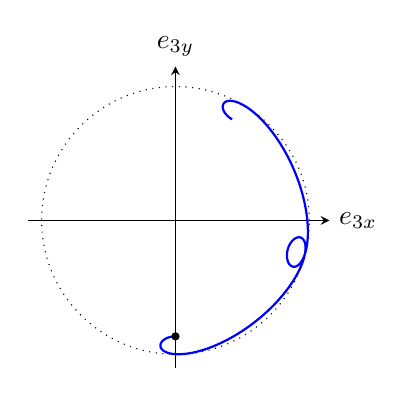
\begin{tikzpicture}[x=1.7cm,y=1.7cm,>=stealth]
\draw[dotted] (0,0) circle (1);\draw[->] (-1.1,0)--(1.15,0) node[right] {$e_{3x}$};\draw[->] (0,-1.1)--(0,1.15) node[above] {$e_{3y}$};
\draw[thick,blue] plot coordinates {(0.000000,-0.866025) (-0.011537,-0.866401) (-0.022962,-0.867524) (-0.034167,-0.869385) (-0.045040,-0.871967) (-0.055472,-0.875246) (-0.065354,-0.879193) (-0.074580,-0.883770) (-0.083043,-0.888935) (-0.090639,-0.894637) (-0.097266,-0.900822) (-0.102824,-0.907425) (-0.107219,-0.914380) (-0.110356,-0.921611) (-0.112147,-0.929039) (-0.112509,-0.936578) (-0.111362,-0.944138) (-0.108635,-0.951624) (-0.104261,-0.958937) (-0.098181,-0.965975) (-0.090347,-0.972633) (-0.080716,-0.978802) (-0.069258,-0.984376) (-0.055951,-0.989243) (-0.040786,-0.993296) (-0.023766,-0.996427) (-0.004904,-0.998533) (0.015770,-0.999512) (0.038216,-0.999269) (0.062379,-0.997715) (0.088189,-0.994766) (0.115563,-0.990351) (0.144406,-0.984404) (0.174608,-0.976873) (0.206044,-0.967716) (0.238582,-0.956906) (0.272075,-0.944428) (0.306367,-0.930280) (0.341294,-0.914478) (0.376683,-0.897049) (0.412359,-0.878039) (0.448140,-0.857507) (0.483843,-0.835525) (0.519285,-0.812183) (0.554285,-0.787580) (0.588667,-0.761830) (0.622258,-0.735057) (0.654896,-0.707396) (0.686425,-0.678990) (0.716703,-0.649988) (0.745599,-0.620544) (0.772995,-0.590819) (0.798788,-0.560971) (0.822891,-0.531161) (0.845233,-0.501548) (0.865757,-0.472287) (0.884427,-0.443529) (0.901219,-0.415419) (0.916126,-0.388095) (0.929157,-0.361685) (0.940337,-0.336310) (0.949701,-0.312079) (0.957302,-0.289090) (0.963200,-0.267432) (0.967468,-0.247179) (0.970189,-0.228397) (0.971453,-0.211137) (0.971357,-0.195440) (0.970005,-0.181336) (0.967503,-0.168842) (0.963963,-0.157966) (0.959497,-0.148705) (0.954220,-0.141047) (0.948247,-0.134969) (0.941692,-0.130441) (0.934665,-0.127425) (0.927279,-0.125872) (0.919640,-0.125732) (0.911851,-0.126943) (0.904013,-0.129441) (0.896220,-0.133154) (0.888564,-0.138006) (0.881129,-0.143917) (0.873996,-0.150803) (0.867240,-0.158576) (0.860927,-0.167143) (0.855122,-0.176410) (0.849881,-0.186280) (0.845253,-0.196652) (0.841284,-0.207425) (0.838010,-0.218494) (0.835463,-0.229752) (0.833667,-0.241091) (0.832641,-0.252403) (0.832396,-0.263576) (0.832937,-0.274497) (0.834262,-0.285056) (0.836364,-0.295138) (0.839227,-0.304630) (0.842829,-0.313419) (0.847141,-0.321392) (0.852128,-0.328437) (0.857749,-0.334444) (0.863955,-0.339304) (0.870691,-0.342911) (0.877895,-0.345163) (0.885499,-0.345961) (0.893431,-0.345210) (0.901612,-0.342823) (0.909956,-0.338716) (0.918374,-0.332815) (0.926774,-0.325052) (0.935058,-0.315370) (0.943125,-0.303722) (0.950873,-0.290070) (0.958197,-0.274390) (0.964994,-0.256670) (0.971157,-0.236912) (0.976585,-0.215131) (0.981177,-0.191358) (0.984836,-0.165639) (0.987469,-0.138036) (0.988992,-0.108625) (0.989324,-0.077501) (0.988395,-0.044771) (0.986144,-0.010558) (0.982519,0.024999) (0.977481,0.061751) (0.971001,0.099535) (0.963065,0.138177) (0.953671,0.177495) (0.942830,0.217298) (0.930568,0.257392) (0.916922,0.297577) (0.901945,0.337652) (0.885702,0.377418) (0.868271,0.416677) (0.849739,0.455238) (0.830206,0.492914) (0.809781,0.529530) (0.788581,0.564919) (0.766729,0.598928) (0.744354,0.631417) (0.721589,0.662262) (0.698571,0.691352) (0.675435,0.718595) (0.652317,0.743916) (0.629353,0.767256) (0.606674,0.788575) (0.584407,0.807848) (0.562673,0.825068) (0.541588,0.840243) (0.521261,0.853397) (0.501791,0.864569) (0.483271,0.873809) (0.465782,0.881181) (0.449399,0.886758) (0.434186,0.890626) (0.420197,0.892875) (0.407476,0.893607) (0.396059,0.892925) (0.385971,0.890940) (0.377229,0.887766) (0.369841,0.883520) (0.363806,0.878318) (0.359114,0.872281) (0.355748,0.865525) (0.353685,0.858168) (0.352892,0.850326) (0.353331,0.842111) (0.354958,0.833634) (0.357722,0.825001) (0.361566,0.816315) (0.366430,0.807676) (0.372246,0.799177) (0.378943,0.790907) (0.386446,0.782952) (0.394674,0.775390) (0.403544,0.768295) (0.412967,0.761736) (0.422851,0.755776)};
\fill (0.000000,-0.866025) circle (1.5pt);
\end{tikzpicture}\\ 回环 $\dot\phi(0)=-0.4000$
\end{minipage}\hfill\begin{minipage}{.46\textwidth}\centering
\begin{tikzpicture}[x=1.7cm,y=1.7cm,>=stealth]
\draw[dotted] (0,0) circle (1);\draw[->] (-1.1,0)--(1.15,0) node[right] {$e_{3x}$};\draw[->] (0,-1.1)--(0,1.15) node[above] {$e_{3y}$};
\draw[thick,blue] plot coordinates {(0.000000,-0.866025) (0.000015,-0.866329) (0.000121,-0.867236) (0.000409,-0.868737) (0.000968,-0.870814) (0.001887,-0.873444) (0.003253,-0.876596) (0.005151,-0.880234) (0.007664,-0.884313) (0.010872,-0.888785) (0.014851,-0.893593) (0.019674,-0.898676) (0.025410,-0.903966) (0.032122,-0.909390) (0.039870,-0.914871) (0.048705,-0.920326) (0.058675,-0.925669) (0.069819,-0.930809) (0.082170,-0.935653) (0.095753,-0.940105) (0.110584,-0.944067) (0.126670,-0.947441) (0.144011,-0.950128) (0.162595,-0.952029) (0.182401,-0.953048) (0.203400,-0.953090) (0.225550,-0.952064) (0.248800,-0.949885) (0.273089,-0.946470) (0.298347,-0.941745) (0.324491,-0.935645) (0.351433,-0.928109) (0.379073,-0.919088) (0.407305,-0.908545) (0.436015,-0.896450) (0.465081,-0.882788) (0.494377,-0.867554) (0.523775,-0.850757) (0.553140,-0.832418) (0.582337,-0.812571) (0.611231,-0.791264) (0.639687,-0.768555) (0.667573,-0.744517) (0.694762,-0.719234) (0.721130,-0.692800) (0.746559,-0.665319) (0.770942,-0.636905) (0.794177,-0.607680) (0.816175,-0.577771) (0.836855,-0.547311) (0.856150,-0.516438) (0.874003,-0.485291) (0.890370,-0.454010) (0.905220,-0.422735) (0.918534,-0.391605) (0.930307,-0.360754) (0.940545,-0.330313) (0.949267,-0.300406) (0.956502,-0.271151) (0.962293,-0.242659) (0.966689,-0.215030) (0.969751,-0.188358) (0.971547,-0.162726) (0.972153,-0.138205) (0.971652,-0.114858) (0.970130,-0.092737) (0.967680,-0.071882) (0.964396,-0.052323) (0.960375,-0.034080) (0.955717,-0.017162) (0.950520,-0.001568) (0.944883,0.012710) (0.938902,0.025692) (0.932674,0.037406) (0.926290,0.047888) (0.919839,0.057179) (0.913406,0.065330) (0.907073,0.072398) (0.900914,0.078444) (0.895001,0.083535) (0.889399,0.087743) (0.884166,0.091144) (0.879356,0.093818) (0.875015,0.095847) (0.871184,0.097315) (0.867896,0.098310) (0.865178,0.098922) (0.863050,0.099239) (0.861526,0.099352) (0.860613,0.099354) (0.860310,0.099334) (0.860609,0.099384) (0.861499,0.099593) (0.862956,0.100051) (0.864956,0.100845) (0.867463,0.102059) (0.870438,0.103778) (0.873833,0.106081) (0.877598,0.109045) (0.881672,0.112745) (0.885992,0.117249) (0.890488,0.122623) (0.895085,0.128928) (0.899704,0.136218) (0.904260,0.144543) (0.908666,0.153946) (0.912829,0.164463) (0.916657,0.176123) (0.920052,0.188948) (0.922917,0.202952) (0.925152,0.218139) (0.926659,0.234507) (0.927339,0.252041) (0.927096,0.270720) (0.925836,0.290513) (0.923470,0.311378) (0.919910,0.333264) (0.915078,0.356111) (0.908900,0.379848) (0.901309,0.404397) (0.892250,0.429669) (0.881673,0.455569) (0.869542,0.481992) (0.855830,0.508828) (0.840522,0.535961) (0.823616,0.563268) (0.805123,0.590624) (0.785065,0.617901) (0.763479,0.644968) (0.740414,0.671696) (0.715933,0.697955) (0.690110,0.723619) (0.663032,0.748564) (0.634797,0.772674) (0.605513,0.795835) (0.575297,0.817945) (0.544274,0.838907) (0.512576,0.858637) (0.480341,0.877059) (0.447711,0.894109) (0.414828,0.909736) (0.381839,0.923898) (0.348887,0.936569) (0.316116,0.947733) (0.283664,0.957389) (0.251666,0.965546) (0.220252,0.972225) (0.189542,0.977459) (0.159650,0.981291) (0.130681,0.983775) (0.102731,0.984973) (0.075884,0.984955) (0.050214,0.983800) (0.025786,0.981589) (0.002651,0.978413) (-0.019150,0.974364) (-0.039586,0.969538) (-0.058640,0.964032) (-0.076301,0.957946) (-0.092573,0.951378) (-0.107468,0.944427) (-0.121005,0.937189) (-0.133216,0.929759) (-0.144138,0.922228) (-0.153818,0.914683) (-0.162308,0.907209) (-0.169668,0.899884) (-0.175962,0.892782) (-0.181262,0.885971) (-0.185641,0.879513) (-0.189179,0.873465) (-0.191958,0.867876) (-0.194062,0.862791) (-0.195579,0.858246) (-0.196598,0.854272) (-0.197210,0.850891) (-0.197506,0.848121) (-0.197577,0.845971) (-0.197515,0.844445) (-0.197411,0.843537) (-0.197357,0.843238)};
\fill (0.000000,-0.866025) circle (1.5pt);
\end{tikzpicture}\\ 尖点 $\dot\phi(0)=0.0000$
\end{minipage}
\par\medskip
\begin{minipage}{.46\textwidth}\centering
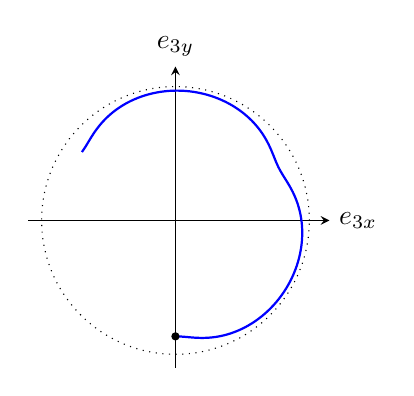
\begin{tikzpicture}[x=1.7cm,y=1.7cm,>=stealth]
\draw[dotted] (0,0) circle (1);\draw[->] (-1.1,0)--(1.15,0) node[right] {$e_{3x}$};\draw[->] (0,-1.1)--(0,1.15) node[above] {$e_{3y}$};
\draw[thick,blue] plot coordinates {(0.000000,-0.866025) (0.010785,-0.866124) (0.021627,-0.866417) (0.032583,-0.866896) (0.043709,-0.867548) (0.055061,-0.868355) (0.066691,-0.869293) (0.078650,-0.870334) (0.090987,-0.871445) (0.103748,-0.872589) (0.116975,-0.873722) (0.130707,-0.874799) (0.144977,-0.875771) (0.159818,-0.876584) (0.175254,-0.877181) (0.191305,-0.877505) (0.207987,-0.877493) (0.225309,-0.877083) (0.243275,-0.876210) (0.261882,-0.874811) (0.281122,-0.872820) (0.300979,-0.870173) (0.321432,-0.866806) (0.342453,-0.862658) (0.364007,-0.857670) (0.386054,-0.851784) (0.408547,-0.844948) (0.431434,-0.837114) (0.454655,-0.828238) (0.478147,-0.818280) (0.501841,-0.807209) (0.525665,-0.794998) (0.549542,-0.781629) (0.573391,-0.767088) (0.597129,-0.751372) (0.620674,-0.734485) (0.643937,-0.716436) (0.666835,-0.697247) (0.689280,-0.676944) (0.711189,-0.655564) (0.732480,-0.633149) (0.753072,-0.609751) (0.772890,-0.585428) (0.791862,-0.560245) (0.809921,-0.534272) (0.827007,-0.507587) (0.843065,-0.480271) (0.858047,-0.452410) (0.871912,-0.424092) (0.884627,-0.395409) (0.896167,-0.366455) (0.906514,-0.337324) (0.915658,-0.308109) (0.923599,-0.278904) (0.930342,-0.249800) (0.935902,-0.220885) (0.940301,-0.192247) (0.943566,-0.163965) (0.945733,-0.136117) (0.946844,-0.108775) (0.946946,-0.082004) (0.946090,-0.055865) (0.944332,-0.030410) (0.941734,-0.005687) (0.938358,0.018267) (0.934269,0.041417) (0.929535,0.063740) (0.924225,0.085218) (0.918406,0.105839) (0.912148,0.125600) (0.905518,0.144503) (0.898583,0.162560) (0.891406,0.179784) (0.884050,0.196198) (0.876573,0.211829) (0.869031,0.226709) (0.861476,0.240874) (0.853955,0.254367) (0.846511,0.267231) (0.839184,0.279516) (0.832006,0.291272) (0.825007,0.302552) (0.818210,0.313413) (0.811634,0.323910) (0.805291,0.334102) (0.799189,0.344047) (0.793330,0.353803) (0.787711,0.363429) (0.782324,0.372981) (0.777154,0.382515) (0.772184,0.392087) (0.767389,0.401747) (0.762741,0.411547) (0.758208,0.421533) (0.753752,0.431749) (0.749332,0.442236) (0.744904,0.453031) (0.740417,0.464165) (0.735823,0.475669) (0.731065,0.487565) (0.726087,0.499871) (0.720831,0.512603) (0.715236,0.525767) (0.709242,0.539367) (0.702786,0.553401) (0.695807,0.567859) (0.688244,0.582728) (0.680036,0.597988) (0.671124,0.613612) (0.661452,0.629569) (0.650967,0.645823) (0.639616,0.662330) (0.627354,0.679042) (0.614139,0.695907) (0.599932,0.712868) (0.584702,0.729861) (0.568424,0.746822) (0.551077,0.763682) (0.532649,0.780368) (0.513135,0.796806) (0.492536,0.812920) (0.470862,0.828634) (0.448131,0.843871) (0.424369,0.858552) (0.399608,0.872604) (0.373891,0.885951) (0.347266,0.898522) (0.319789,0.910251) (0.291525,0.921072) (0.262542,0.930928) (0.232917,0.939763) (0.202731,0.947530) (0.172071,0.954189) (0.141027,0.959703) (0.109693,0.964047) (0.078164,0.967200) (0.046538,0.969151) (0.014912,0.969895) (-0.016614,0.969437) (-0.047945,0.967789) (-0.078987,0.964969) (-0.109646,0.961006) (-0.139835,0.955933) (-0.169471,0.949790) (-0.198474,0.942626) (-0.226773,0.934493) (-0.254300,0.925449) (-0.280995,0.915556) (-0.306807,0.904881) (-0.331689,0.893492) (-0.355605,0.881463) (-0.378524,0.868865) (-0.400425,0.855774) (-0.421293,0.842263) (-0.441122,0.828408) (-0.459913,0.814281) (-0.477674,0.799954) (-0.494420,0.785495) (-0.510172,0.770971) (-0.524958,0.756444) (-0.538812,0.741974) (-0.551772,0.727616) (-0.563881,0.713418) (-0.575186,0.699428) (-0.585738,0.685685) (-0.595590,0.672223) (-0.604800,0.659073) (-0.613426,0.646258) (-0.621526,0.633797) (-0.629162,0.621702) (-0.636395,0.609980) (-0.643284,0.598632) (-0.649891,0.587655) (-0.656273,0.577038) (-0.662489,0.566769) (-0.668594,0.556825) (-0.674640,0.547184) (-0.680679,0.537816) (-0.686757,0.528688) (-0.692918,0.519762) (-0.699202,0.510996)};
\fill (0.000000,-0.866025) circle (1.5pt);
\end{tikzpicture}\\ 单向 $\dot\phi(0)=0.3000$
\end{minipage}\hfill\begin{minipage}{.46\textwidth}\centering
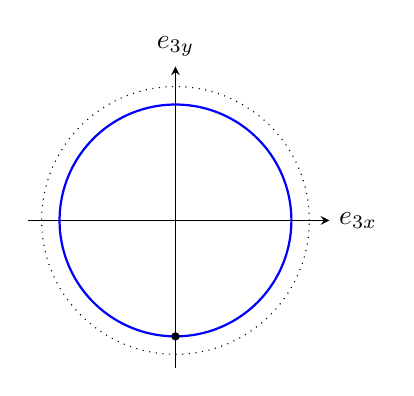
\begin{tikzpicture}[x=1.7cm,y=1.7cm,>=stealth]
\draw[dotted] (0,0) circle (1);\draw[->] (-1.1,0)--(1.15,0) node[right] {$e_{3x}$};\draw[->] (0,-1.1)--(0,1.15) node[above] {$e_{3y}$};
\draw[thick,blue] plot coordinates {(0.000000,-0.866025) (0.036265,-0.865266) (0.072467,-0.862988) (0.108542,-0.859197) (0.144426,-0.853898) (0.180057,-0.847101) (0.215372,-0.838818) (0.250309,-0.829063) (0.284807,-0.817854) (0.318805,-0.805210) (0.352244,-0.791154) (0.385065,-0.775709) (0.417211,-0.758904) (0.448625,-0.740767) (0.479251,-0.721331) (0.509037,-0.700629) (0.537930,-0.678698) (0.565879,-0.655577) (0.592835,-0.631305) (0.618751,-0.605926) (0.643582,-0.579484) (0.667284,-0.552025) (0.689815,-0.523598) (0.711136,-0.494252) (0.731209,-0.464040) (0.750000,-0.433013) (0.767475,-0.401226) (0.783603,-0.368736) (0.798357,-0.335598) (0.811710,-0.301872) (0.823639,-0.267617) (0.834123,-0.232891) (0.843144,-0.197758) (0.850686,-0.162277) (0.856735,-0.126512) (0.861281,-0.090524) (0.864317,-0.054378) (0.865835,-0.018137) (0.865835,0.018137) (0.864317,0.054378) (0.861281,0.090524) (0.856735,0.126512) (0.850686,0.162277) (0.843144,0.197758) (0.834123,0.232891) (0.823639,0.267617) (0.811710,0.301872) (0.798357,0.335598) (0.783603,0.368736) (0.767475,0.401226) (0.750000,0.433013) (0.731209,0.464040) (0.711136,0.494252) (0.689815,0.523598) (0.667284,0.552025) (0.643582,0.579484) (0.618751,0.605926) (0.592835,0.631305) (0.565879,0.655577) (0.537930,0.678698) (0.509037,0.700629) (0.479251,0.721331) (0.448625,0.740767) (0.417211,0.758904) (0.385065,0.775709) (0.352244,0.791154) (0.318805,0.805210) (0.284807,0.817854) (0.250309,0.829063) (0.215372,0.838818) (0.180057,0.847101) (0.144426,0.853898) (0.108542,0.859197) (0.072467,0.862988) (0.036265,0.865266) (0.000000,0.866025) (-0.036265,0.865266) (-0.072467,0.862988) (-0.108542,0.859197) (-0.144426,0.853898) (-0.180057,0.847101) (-0.215372,0.838818) (-0.250309,0.829063) (-0.284807,0.817854) (-0.318805,0.805210) (-0.352244,0.791154) (-0.385065,0.775709) (-0.417211,0.758904) (-0.448625,0.740767) (-0.479251,0.721331) (-0.509037,0.700629) (-0.537930,0.678698) (-0.565879,0.655577) (-0.592835,0.631305) (-0.618751,0.605926) (-0.643582,0.579484) (-0.667284,0.552025) (-0.689815,0.523598) (-0.711136,0.494252) (-0.731209,0.464040) (-0.750000,0.433013) (-0.767475,0.401226) (-0.783603,0.368736) (-0.798357,0.335598) (-0.811710,0.301872) (-0.823639,0.267617) (-0.834123,0.232891) (-0.843144,0.197758) (-0.850686,0.162277) (-0.856735,0.126512) (-0.861281,0.090524) (-0.864317,0.054378) (-0.865835,0.018137) (-0.865835,-0.018137) (-0.864317,-0.054378) (-0.861281,-0.090524) (-0.856735,-0.126512) (-0.850686,-0.162277) (-0.843144,-0.197758) (-0.834123,-0.232891) (-0.823639,-0.267617) (-0.811710,-0.301872) (-0.798357,-0.335598) (-0.783603,-0.368736) (-0.767475,-0.401226) (-0.750000,-0.433013) (-0.731209,-0.464040) (-0.711136,-0.494252) (-0.689815,-0.523598) (-0.667284,-0.552025) (-0.643582,-0.579484) (-0.618751,-0.605926) (-0.592835,-0.631305) (-0.565879,-0.655577) (-0.537930,-0.678698) (-0.509037,-0.700629) (-0.479251,-0.721331) (-0.448625,-0.740767) (-0.417211,-0.758904) (-0.385065,-0.775709) (-0.352244,-0.791154) (-0.318805,-0.805210) (-0.284807,-0.817854) (-0.250309,-0.829063) (-0.215372,-0.838818) (-0.180057,-0.847101) (-0.144426,-0.853898) (-0.108542,-0.859197) (-0.072467,-0.862988) (-0.036265,-0.865266) (-0.000000,-0.866025)};
\fill (0.000000,-0.866025) circle (1.5pt);
\end{tikzpicture}\\ 稳态 $\dot\phi(0)=0.5858$
\end{minipage}
\caption{陀螺轴单位向量的水平投影. 无量纲$I=k=1$, $b=2$, $\theta(0)=\pi/3$, $\dot\theta(0)=\phi(0)=0$; 每幅由其给定初始进动率确定$a,E_*$. 非稳态图显示两个章动周期, 稳态图显示一圈. 黑点为初始位置, 蓝线由本节解析方程数值积分采样, 不把图形采样当成全部初值的证明.}
\end{figure}

\begin{example}
\textbf{水平稳态进动的稳定性.} 
固定$a,b$, 检查$\theta_0=\pi/2$的稳态, 并取无量纲$I=k=1$, $b=2$作数值例.
\end{example}
\begin{solution}
在水平位置$\dot\phi=a/I$. 由稳态方程$-b\dot\phi+k=0$, 必须$a=Ik/b$. 直接对有效势微分, 有$V'(\pi/2)=ab/I-k=0$, $V''(\pi/2)=(a^2+b^2)/I>0$. 因而固定两个循环动量下的小章动$\eta=\theta-\pi/2$满足$I\ddot\eta+V''(\pi/2)\eta=0$, 稳定且频率为$\sqrt{a^2+b^2}/I$. 例中$a=1/2$, 进动率$1/2$, 小章动频率$\sqrt{17}/2$. 这证明的是倾角方向的局部稳定; 两个循环角的初始相位可自由改变, 不要求所有相位扰动回到同一个时刻的同一个轴尖位置.
\end{solution}

竖直向上的“睡眠陀螺”还可检查极点退化. 要趋近$\theta=0$必须$a=b$. 此时
$V=b^2(1-\cos\theta)/[2I(1+\cos\theta)]+k\cos\theta
=k+(b^2/(8I)-k/2)\theta^2+O(\theta^4)$.
故$b^2>4Ik$时倾斜有回复力,$b^2<4Ik$时竖直状态不稳定. 临界$b^2=4Ik$时二次项消失, 不能由线性化宣称稳定或不稳定; 此时用$1-\cos\theta=2\sin^2(\theta/2)$精确展开得到正的四次项$k\theta^4/8+O(\theta^6)$, 是非线性退化极小值. 在固定$a=b$的约化模型里仍有能量局部稳定, 但线性频率为零.

新增内容来源: 8.09第2章第30--36、43、46--51页. 轴角证明、坐标约定核对、两种进动率的空间推导、水平稳定例与临界四次项为本册独立推导; 原稿角点立方体的简并惯量印误已纠正.


本章来源: 8.09第2章. 角度约定、惯性张量正定性、平行轴推导和稳定条件说明为中文补充.
